%%%%%%%% ICML 2026 — WORKING DRAFT (v5) %%%%%%%%%%%%%%%%%
\documentclass{article}

\usepackage{microtype}
\usepackage{graphicx}
\usepackage{booktabs}
\usepackage{hyperref}

% arXiv preprint version: [preprint] shows the real author block and prints a
% neutral "Preprint." footer -- it does NOT print the [accepted] option's
% "Proceedings of ... ICML" line, so it makes no claim of publication.
\usepackage[preprint]{icml2026}

\usepackage{amsmath}
\usepackage{amssymb}

% --- Float placement tuning (does not alter ICML page style) -------------
% The paper is float-heavy; by default LaTeX lets two full-width (table*/figure*)
% floats stack at the top of one page and lets a page be almost all floats.
% These settings spread the full-width tables onto separate pages and force a
% little body text onto every page so floats de-clump.
\setcounter{dbltopnumber}{1}            % at most one full-width float per page top
\renewcommand{\dbltopfraction}{0.85}    % a single wide table may use most of the top
\renewcommand{\textfraction}{0.12}      % keep a sliver of text on every page
\renewcommand{\floatpagefraction}{0.80} % avoid sparse float-only pages

% Courier (pcr) TFMs are absent from this minimal TeX install; route \texttt to
% Computer Modern typewriter, which is always present.
\renewcommand{\ttdefault}{cmtt}

\icmltitlerunning{Cost-Effective Judging of AI-Generated Proofs}

\begin{document}

\twocolumn[
  \icmltitle{Cost-Effective Automated Judging of\\
    Natural-Language Mathematical Proofs}

  \icmlsetsymbol{equal}{*}

  \begin{icmlauthorlist}
    \icmlauthor{Benjamin Grayzel}{dartmouth}
  \end{icmlauthorlist}

  \icmlaffiliation{dartmouth}{Department of Computer Science, Dartmouth College, Hanover, NH, USA}

  \icmlcorrespondingauthor{Benjamin Grayzel}{\mbox{benjamin.a.grayzel.gr@dartmouth.edu}, \mbox{benjamingrayzel@gmail.com}}

  \icmlkeywords{LLM-as-a-judge, mathematical reasoning, natural language proof grading, cost-efficiency, open-weight models}

  \vskip 0.3in
]

\printAffiliationsAndNotice{}

\begin{abstract}
  Grading natural-language mathematical proofs is a recurring cost in evaluating
  math-reasoning systems, and frontier LLM judges are expensive. We ask whether
  cheap open-weight models can serve as reliable judges given a candidate proof, a
  ground-truth proof, and a human-grading rubric. On a 200-instance validation
  sample of IMO-GradingBench, three cheap judges (GPT-OSS-120B, DeepSeek-V4-Flash,
  Gemma-4-31B) agree with human pass/fail decisions at rates statistically
  indistinguishable from Claude Opus 4.7 and Gemini 3.1 Pro, at up to $100\times$
  lower cost. We had expected a majority vote of the three to be the best budget
  option; it matched the frontier but did not improve on its strongest member.
  Extending to the full 1000-instance benchmark and exploring consensus rules, we
  found that requiring unanimous agreement (all-three-pass) reaches the highest
  pass-agreement and precision and, on four replicate runs, the smallest
  run-to-run spread. The headline finding is that cheap judges are competitive
  with the frontier at one to two orders of magnitude lower cost; as a deployable
  default we recommend all-three-pass, with the caveat that this rule was
  identified post-hoc and warrants independent replication.
\end{abstract}

\section{Introduction}
\label{sec:intro}

Benchmarks for AI mathematical reasoning increasingly include problems whose
solutions are full natural-language proofs rather than short final answers, and
scoring those proofs is a bottleneck. Formal verification with proof assistants
such as Lean \citep{moura2021lean} gives trustworthy guarantees and has
reached IMO-medal performance with AlphaProof \citep{hubert2025alphaproof}. Extending it to the breadth of
research mathematics, through autoformalization and self-evolving provers, is an
active frontier; until that coverage arrives, most proofs are still graded in
natural language, as the 2025 IMO gold-medal results from frontier models were.

While the model under study can change between experiments, the judge must be
reliable and held fixed across an entire study, so its cost is a tax on the whole
research effort, and frontier judges are expensive. The same cost recurs inside
self-improving systems, where a loop that generates, critiques, and revises
proofs needs a judgment at every step, so an expensive judge limits how much such
a system can iterate. This motivates a concrete question: \emph{is there a cheap
judge a budget-constrained researcher can trust for proof grading?}

We study this judging task on \textbf{IMO-GradingBench} \citep{luong2025robust}, the
grading split of IMO-Bench: 1{,}000 instances, each pairing an Olympiad problem
and a reference solution with a candidate proof and an expert human grade on the
standard 0--7 IMO scale. The judge reads the problem, reference, and candidate,
and predicts the grade. We are deliberately narrow in scope; this is a study of
\emph{judging}, not \emph{solving}, on problems that come with a reference proof
and a human grade (not reference-free verification).

Our prior expectation, following the Panel-of-LLM-evaluators result
\citep{verga2024poll}, was that a (majority-vote) consensus of several cheap models would be
the safest choice, as offsetting biases should cancel. We tested this: the
consensus performed well, but it did not beat the strongest individual model
within it. The more useful and general finding is that the cheap tier as a whole
is competitive: cheap open-weight judges match frontier baselines (Claude Opus
4.7, Gemini 3.1 Pro) on pass/fail agreement with human graders at a
\textbf{cost of 1--2 orders of magnitude lower} in our setup. In a post-hoc rule
search on the full benchmark we found that the unanimous variant (all-three-pass)
of the same trio outperformed both cheap and frontier judges (on pass-agreement,
precision, and stability) and is the configuration we recommend pending
replication.

\section{Related Work}
\label{sec:related}

LLM-as-a-judge \citep{zheng2023judging} is now the standard tool but is known to
exhibit position, verbosity, and self-preference biases and to be sensitive to
prompt design \citep{gu2024survey}. For proofs specifically, frontier models often
fail to produce valid arguments even when their final answers are correct
\citep{petrov2025proof}, motivating dedicated grading benchmarks such as the Open Proof
Corpus \citep{dekoninck2025opc} and IMO-GradingBench \citep{luong2025robust}. Cost
has received less attention: \citet{verga2024poll} show that small-model panels can
outperform a single large judge at roughly $7\times$ lower cost on QA and chatbot
tasks.

Two concurrent works frame our contribution. \citet{ma2026proofgrader} search the
evaluator design space and reach expert-level agreement by combining a strong
reasoning backbone with reference solutions, marking schemes, and ensembling; we
ask whether the backbone itself must be strong and find that, for reference-based
pass/fail grading, it need not be. \citet{naik2026frontier} study the closest
reference-\emph{free} version of our question and report cheap judges trailing the
frontier by ${\sim}10\%$ in accuracy (and ${\sim}25\%$ in self-consistency), a
gap that prompt ensembling narrows. In our reference-\emph{based} setting (judging
against ground-truth solutions), the accuracy gap closes entirely. This is
consistent with the reference solution doing work the judge would otherwise have
to do. We do not measure self-consistency, which remains open.

\section{Problem Setting}
\label{sec:setting}

We consider grading instances of the form \emph{(problem, ground-truth solution,
candidate solution, human score)}. A judge reads the first three and outputs a
score; we compare its score to the human's. The decision that matters most for
downstream use is the \textbf{pass/fail boundary}: did the candidate proof meet
the bar (a score of $\geq 6$ on the 0--7 IMO scale)? Our primary metric is
\textbf{pass-agreement}: the fraction of instances where the judge's pass/fail
decision matches the human's. We report precision, recall, and F1 at that
boundary, and Spearman rank correlation with the human score as a secondary,
ordinal measure (appropriate for the coarse $\{0, 1, 6, 7\}$ output). We also
report per-grading cost.

\section{Methodology}
\label{sec:method}

\paragraph{Data and sampling.}
From IMO-GradingBench's 1{,}000 instances (spanning 30 IMO-style problems), we
draw two disjoint random samples of 200 by uniform selection without replacement:
a \emph{prior} (exploratory) sample with seed 42, used for exploration and for
selecting the consensus trio, and a \emph{validation} sample with seed 7, drawn
from the remaining 800 instances, used as a clean held-out test.
Section~\ref{sec:full} additionally reports results over the complete
1{,}000-instance benchmark. All headline results are on the validation sample
unless noted otherwise.

\paragraph{Judge prompt and scoring buckets.}
Every judge uses the same prompt and is instructed to emit a score in
$\{0, 1, 6, 7\}$ (incorrect / partial / almost / correct); our parser accepts any
integer 0--7, and a handful of off-bucket scores (4 across all runs, under 0.1\%)
occurred and are scored as parsed. This four-bucket scheme follows the public grading
prompt released with IMO-GradingBench \citep{luong2025robust}, which we lightly adapt
so that our judges are scored under an established, externally defined rubric
rather than one of our own design. Pass/fail and all confusion-matrix metrics use
the raw human score, so a human-4 graded as 6 by a judge is correctly counted as
a false positive. The benchmark also ships a per-problem marking scheme; we do not
provide it to the judge.

\paragraph{Judges and reasoning settings.}
We evaluate three cheap open-weight models (\textbf{GPT-OSS-120B},
\textbf{DeepSeek-V4-Flash}, and \textbf{Gemma-4-31B}) and two frontier baselines,
\textbf{Claude Opus 4.7} and \textbf{Gemini 3.1 Pro}. The three cheap models were
chosen for their cost-accuracy tradeoff and offsetting calibration biases (Gemma
over-credits, DeepSeek-V4-Flash under-credits), the intended ingredient for a
majority vote. These bias signs hold across our replicate runs
(Section~\ref{sec:variance}), so the trio's diversity is a property of the models,
not of any single run. \emph{For each model we use the strongest reasoning
configuration it exposes.} These settings are not normalized and are not directly
comparable across providers: GPT-OSS-120B runs at effort \texttt{xhigh},
Gemma-4-31B and Gemini-3.1-Pro with reasoning activated (listed as effort
\texttt{high}), while Claude Opus 4.7 (adaptive thinking) and DeepSeek-V4-Flash
(default) self-regulate their reasoning, so we report them at their default. The
``Reasoning'' column in each table names the per-model setting.

\paragraph{Consensus rule.}
The cheap consensus is the majority pass/fail vote of the three cheap models. We
also report a \emph{continuous} consensus score (the mean of member scores) only
for completeness: because averaging the bucketed $\{0, 1, 6, 7\}$ outputs produces
intermediate values that no single judge can emit, the consensus Spearman $\rho$
is not comparable to single-judge correlations, and we therefore omit it (shown as
``---'') throughout. Majority vote was the pre-specified consensus rule; alternate
variants (pairs, all-three-pass) were added during the full-benchmark analysis in
Section~\ref{sec:full} after observing that the vote did not improve over its
strongest member on validation.

\paragraph{Providers, coverage, and re-runs.}
The cheap open-weight judges are served through OpenRouter by a shifting pool of
third-party providers at varying quantizations; we did not pin a provider, so a
single judge's pass-agreement can move by a few points between runs (quantified in
Section~\ref{sec:variance}). For a reproducible number, pin a provider and log the
served-provider field; the frontier baselines are first-party, single-provider,
and stable. Under $2\%$ of judge calls failed to return a parseable score on the
first attempt (transient rate limits, or reasoning that exceeded the 32k-token
output ceiling without concluding); we re-ran these (runaways usually converged on
a retry) and never substituted fabricated scores. Final coverage is 1000/1000 for
each cheap judge and 200/200 for each frontier baseline. All per-instance scores
and standalone code (standard library only) that regenerates every table and
figure are in the supplementary materials.

\section{Results}
\label{sec:results}

Table~\ref{tab:main} reports the validation results, sorted by pass-agreement,
with $95\%$ bootstrap confidence intervals (1000 resamples). This is our primary
comparison: the only setting in which all five judges, frontier and cheap, are run
head-to-head. Figure~\ref{fig:forest} shows the same comparison as a forest plot.

\begin{table*}[t]
  \caption{Validation results ($n=200$; metrics over valid responses). Reasoning
    names each model's maximum/natural setting (see Section~\ref{sec:method}); the
    consensus Spearman $\rho$ is omitted (``---'') as it is not comparable to
    single-judge correlations.}
  \label{tab:main}
  \begin{center}
    \begin{small}
      \begin{tabular}{llccccccr}
        \toprule
        Judge & Reasoning & Pass-agree [95\% CI] & Prec. & Rec. & F1 & Spearman $\rho$ & Cost / 200 \\
        \midrule
        GPT-OSS-120B           & \texttt{xhigh}    & 0.875 [0.830, 0.920] & 0.722 & 0.912 & 0.806 & 0.623 & \textbf{\$0.32} \\
        DeepSeek-V4-Flash      & default           & 0.860 [0.815, 0.910] & 0.738 & 0.789 & 0.763 & 0.660 & \$0.70 \\
        Cheap consensus (trio) & ---               & 0.855 [0.810, 0.905] & 0.689 & 0.895 & 0.779 & ---   & \$1.73 \\
        Claude Opus 4.7        & adaptive          & 0.855 [0.805, 0.900] & 0.680 & 0.930 & 0.785 & \textbf{0.715} & \$32.45 \\
        Gemini 3.1 Pro         & \texttt{high}     & 0.840 [0.790, 0.890] & 0.662 & 0.895 & 0.761 & 0.704 & \$28.61 \\
        Gemma-4-31B            & \texttt{high}     & 0.795 [0.740, 0.850] & 0.591 & 0.912 & 0.717 & 0.676 & \$0.71 \\
        \bottomrule
      \end{tabular}
    \end{small}
  \end{center}
  \vskip -0.1in
\end{table*}

\begin{figure}[t]
  \centering
  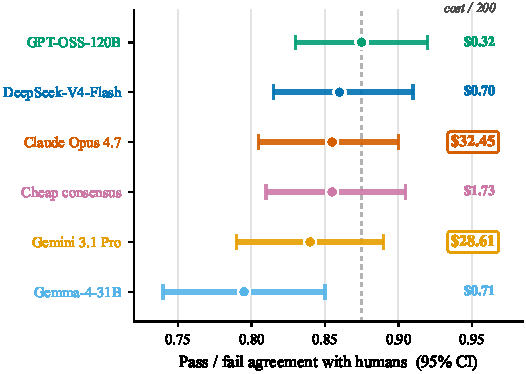
\includegraphics[width=\columnwidth]{../../supplement/results/figures/figure1_forest.pdf}
  \caption{Pass/fail agreement with humans (95\% CI) for all six systems (the five
    judges and the cheap consensus) on the validation sample ($n=200$), sorted by
    point estimate, with per-200-call cost at right (frontier costs boxed). Every
    cheap judge's interval overlaps the leader's estimate (dashed line), at one to
    two orders of magnitude lower cost than the frontier baselines.}
  \label{fig:forest}
\end{figure}

\paragraph{The cheap tier is competitive with the frontier.}
The confidence intervals for the top five systems (all but Gemma) overlap
substantially. GPT-OSS-120B has the highest point estimate, but it is best read as
the front-runner of a cluster, not a clear winner: pairwise, it is statistically
indistinguishable from Claude Opus 4.7 ($P \approx 0.76$ of being higher on a
resample) and only weakly separated from Gemma. Our sample does not support a
claim that any single model is best. It does support the claim that the cheap
cluster sits inside the frontier's interval: three open-weight judges, each costing
under \$1 per 200 gradings, match two models costing \$28--32 for the same work.

\paragraph{The consensus did not beat its best member.}
The majority vote matched Opus on pass-agreement, but its agreement ($0.855$) and
F1 ($0.779$) fell below those of its strongest single member, GPT-OSS-120B
($0.875$, $0.806$), at roughly five times the cost (\$1.73 vs \$0.32). Combining a
strong model with two weaker ones diluted rather than improved the result. We
return in Section~\ref{sec:full} to whether a different consensus rule over the
same trio fares better.

\paragraph{The price gap is dramatic.}
GPT-OSS-120B grades at \$0.0016 per instance, about \textbf{$100\times$ cheaper
than Claude Opus 4.7} (\$0.162) and ${\sim}90\times$ cheaper than Gemini 3.1 Pro at
high reasoning (\$0.143). Every cheap judge in Table~\ref{tab:main} is one to two
orders of magnitude cheaper than either frontier baseline, with no consistent
accuracy penalty on the pass/fail decision. This is the practical headline.

\paragraph{Where the frontier still leads.}
The frontier keeps an edge on rank correlation with the human score: Opus ($0.715$)
and Gemini ($0.704$) sit above the cheap judges ($0.62$--$0.68$). The margin is
modest (Gemma reaches $0.676$), but for applications that need a graded quality
signal rather than a pass/fail gate, a frontier judge is still the safer choice.
Appendix~\ref{app:correlation} visualizes this split.

\paragraph{All of this is relative.}
In absolute terms no judge here is highly reliable: single-judge precision and F1
sit in the $0.6$--$0.8$ range, and because only ${\sim}30\%$ of instances are
passes, the high pass-agreement rates are less impressive than they appear (a
fail-everything baseline already scores $0.715$). Pushing precision into the
mid-$0.80$s takes the unanimous consensus rules of Section~\ref{sec:full}.

\medskip
Reasoning effort turns out to be a model-specific lever: raising Gemini to high
reasoning does not change its agreement, while it matters a great deal for
GPT-OSS-120B; we report this comparison in Appendix~\ref{app:reasoning}.

\section{Additional Results}
\label{sec:additional}

The two studies below extend the primary comparison. Neither changes the headline,
and both are run on the cheap tier only (the frontier baselines are
validation-only, for budget); we present them as supporting evidence.

\subsection{The full benchmark ($n=1000$)}
\label{sec:full}

We graded all three cheap judges over the \textbf{complete 1000-instance
benchmark} (prior + validation + the remaining 600) for a more stable estimate and
to explore consensus configurations beyond the pre-specified majority vote.

\begin{table*}[t]
  \caption{Full benchmark ($n=1000$), 95\% bootstrap CIs (2000 resamples). Pairs
    and ``all-three'' use the unanimous-pass rule (a candidate passes only if all
    listed members pass); consensus Spearman $\rho$ is omitted (``---''; see
    Section~\ref{sec:method}).}
  \label{tab:full}
  \begin{center}
    \begin{small}
      \begin{tabular}{lccccc}
        \toprule
        System & Pass-agree [95\% CI] & Prec. & Rec. & F1 & Spearman $\rho$ \\
        \midrule
        \multicolumn{6}{l}{\emph{Individual models}} \\
        DeepSeek-V4-Flash      & 0.873 [0.853, 0.893] & 0.815 & 0.812 & 0.814 & 0.732 \\
        GPT-OSS-120B (\texttt{xhigh}) & 0.842 [0.818, 0.864] & 0.716 & 0.889 & 0.793 & 0.704 \\
        Gemma-4-31B (\texttt{high})   & 0.801 [0.775, 0.825] & 0.640 & 0.953 & 0.766 & 0.741 \\
        \addlinespace
        \multicolumn{6}{l}{\emph{Pairs (unanimous pass)}} \\
        DeepSeek + GPT-OSS     & 0.878 [0.858, 0.897] & 0.852 & 0.777 & 0.813 & --- \\
        DeepSeek + Gemma       & 0.877 [0.857, 0.897] & 0.824 & 0.812 & 0.818 & --- \\
        GPT-OSS + Gemma        & 0.866 [0.844, 0.887] & 0.765 & 0.877 & 0.817 & --- \\
        \addlinespace
        \multicolumn{6}{l}{\emph{Combined}} \\
        Majority vote (trio)   & 0.863 [0.841, 0.883] & 0.744 & 0.912 & 0.819 & --- \\
        All-three-pass         & 0.879 [0.859, 0.898] & 0.855 & 0.777 & 0.814 & --- \\
        \bottomrule
      \end{tabular}
    \end{small}
  \end{center}
  \vskip -0.1in
\end{table*}

Three observations. First, \textbf{the single-model leader changes with scale}:
GPT-OSS-120B led on the 200-instance validation sample, but on the full benchmark
DeepSeek-V4-Flash is the strongest single judge ($0.873$ vs $0.842$), direct
evidence that 200 instances cannot separate the leaders (Figure~\ref{fig:leaderflip}).
Second, \textbf{the choice of consensus rule trades precision against recall}: the
unanimous all-three-pass rule reaches the highest pass-agreement ($0.879$) and
precision ($0.855$), while majority vote is the most recall-heavy ($0.912$). Third,
\textbf{every confidence interval still overlaps}, consistent with the validation
finding that no single configuration is separable.

\begin{figure}[t]
  \centering
  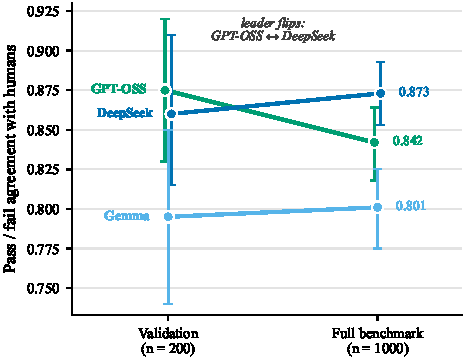
\includegraphics[width=\columnwidth]{../../supplement/results/figures/figure2_leader_flip.pdf}
  \caption{The strongest single judge flips between the 200-instance validation
    sample and the full 1000-instance benchmark (GPT-OSS $\leftrightarrow$
    DeepSeek); the 95\% CIs overlap throughout, so 200 instances cannot separate the
    leaders.}
  \label{fig:leaderflip}
\end{figure}

The choice of consensus rule is effectively a precision/recall dial
(Figure~\ref{fig:prdial}). Unanimous rules, such as both-pass pairs (e.g., DeepSeek
+ GPT-OSS) or all-three-pass, suppress false positives by passing a candidate only
when members agree, which is the right profile when wrongly passing a flawed proof
is costly; majority vote instead maximizes recall. The strictness of a pair is
driven by its most conservative member: any pairing that includes the
under-crediting DeepSeek-V4-Flash inherits high precision, and adding the
over-crediting Gemma to an already-strict pair changes little.

\begin{figure}[t]
  \centering
  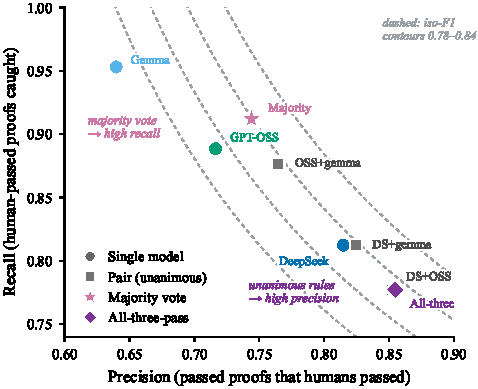
\includegraphics[width=\columnwidth]{../../supplement/results/figures/figure3_precision_recall.pdf}
  \caption{Consensus rule as a precision/recall dial on the full benchmark
    ($n=1000$); dashed lines are iso-F1 contours. Majority vote sits at high recall,
    while the unanimous rules (both-pass pairs and all-three-pass) move toward high
    precision.}
  \label{fig:prdial}
\end{figure}

\subsection{Run-to-run variance (validation, four runs)}
\label{sec:variance}

How stable are these numbers across repeated runs? We re-ran the cheap tier on the
same 200-instance validation sample three more times, with no fixed random seed,
giving four independent runs per system (including the original).
Table~\ref{tab:runstab} reports pass-agreement for each run, with the mean and
standard deviation; Figure~\ref{fig:runstability} plots the per-run points and their
spread.

\begin{table*}[t]
  \caption{Run-to-run pass-agreement on validation ($n=200$). \emph{orig}--\emph{rep3}
    are four independent runs; \emph{mean} and \emph{std} are over those four.
    \emph{Self-maj.} and \emph{self-all-3} apply the consensus rules to one model's
    own three replicates (rep1--3), over the problems where all three are valid
    ($n=191$--$199$): self-maj.\ passes if $\geq 2$ of 3 runs pass, self-all-3 if all 3
    pass. Consensus-of-consensus cells are blank (``---'').}
  \label{tab:runstab}
  \begin{center}
    \begin{small}
      \setlength{\tabcolsep}{4.5pt}
      \begin{tabular}{lcccccccc}
        \toprule
        System & orig & rep1 & rep2 & rep3 & mean & std & Self-maj. & Self-all-3 \\
        \midrule
        DeepSeek-V4-Flash      & 0.860 & 0.861 & 0.898 & 0.905 & 0.881 & 0.024 & 0.901 & 0.895 \\
        GPT-OSS-120B \texttt{xhigh} & 0.875 & 0.863 & 0.829 & 0.835 & 0.851 & 0.022 & 0.847 & 0.888 \\
        Gemma-4-31B \texttt{high}   & 0.795 & 0.820 & 0.810 & 0.814 & 0.810 & 0.011 & 0.824 & 0.849 \\
        Majority vote (trio)   & 0.855 & 0.875 & 0.890 & 0.875 & 0.874 & 0.014 & --- & --- \\
        \textbf{All-three-pass} & 0.895 & 0.895 & 0.903 & 0.915 & \textbf{0.902} & \textbf{0.009} & --- & --- \\
        \bottomrule
      \end{tabular}
    \end{small}
  \end{center}
  \vskip -0.1in
\end{table*}

\begin{figure}[t]
  \centering
  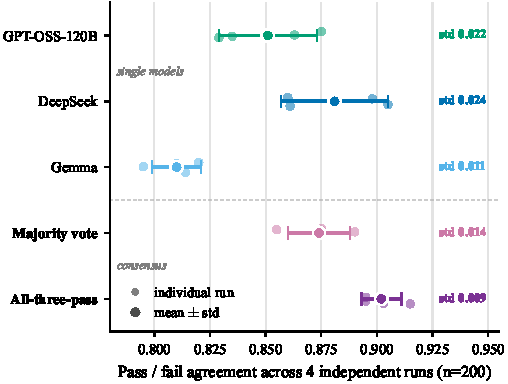
\includegraphics[width=\columnwidth]{../../supplement/results/figures/figure4_run_stability.pdf}
  \caption{Run-to-run pass-agreement across four independent runs ($n=200$). Faded
    points are individual runs; solid points are mean $\pm$ std. All-three-pass is
    both the highest and the tightest; single cheap judges drift more than the
    consensus rules.}
  \label{fig:runstability}
\end{figure}

Three points. First, \textbf{the unanimous all-three-pass rule is the best
configuration on this sample on both counts}: the highest mean ($0.902$) and the
smallest spread (std $0.009$). Second, \textbf{the majority vote is steadier than
its individual members} (std $0.014$, versus $0.022$--$0.024$ for GPT-OSS and
DeepSeek). Third, the single-judge numbers move enough to matter:
\textbf{GPT-OSS's headline $0.875$ is the top of its $0.83$--$0.88$ range, not a
fixed value}, while DeepSeek is the most reliable single judge (mean $0.881$),
matching the full-benchmark result in Section~\ref{sec:full}. We do not claim
consensus always reduces variance: Gemma alone is the steadiest single judge (std
$0.011$), edging out even the majority vote.

This variance comes from how the models are served, not from the models changing.
Each call to GPT-OSS-120B or DeepSeek-V4-Flash is routed to one of several
third-party providers, and different providers run the model at different numerical
precisions (quantization), so identical requests can return slightly different
scores. Gemma is served almost entirely (${\sim}93\%$) by a single provider, which
is likely why its spread is small. The frontier baselines run on their own
providers and are stable (a 20-problem re-run of Opus produced no pass/fail
changes), so the run-to-run movement is specific to the cheaply-hosted open judges
and does not affect the head-to-head comparison in Section~\ref{sec:results}. It
does mean that any single cheap-judge number should be read as one draw from a
few-point band, which is a further reason to prefer the steadier consensus rules.

The two rightmost columns of Table~\ref{tab:runstab} turn that variance to
advantage by applying the consensus rules to a single model's own three runs. For
the recall-biased judges this helps: requiring all three GPT-OSS runs to pass lifts
agreement from a single-run mean of $0.851$ to $0.888$, and Gemma from $0.810$ to
$0.849$, because the run-to-run noise produces occasional spurious passes that a
unanimity rule filters out, lifting GPT-OSS's precision from $0.72$ to $0.78$ and
giving it its highest F1 ($0.81$). DeepSeek, already balanced, does not surpass its
best single run ($0.905$). This is the same precision-for-recall trade as the
cross-model rules in Section~\ref{sec:full}, amplified because successive runs are
often served by different providers; in effect, running one cheap model three times
and requiring unanimity recovers much of the multi-model consensus benefit (GPT-OSS
self-all-3 reaches $0.888$, approaching the cross-model all-three-pass at $0.902$).
This is why we recommend all-three-pass as the default budget judge: within noise of
every alternative on agreement, but the most precise and the most stable, and cheap
enough that the single-model variant is a viable fallback when three judges is too
many calls.

\section{Limitations}
\label{sec:limits}

\textbf{Sample size and intervals.} Even on the full benchmark, the leading
systems' confidence intervals overlap and we cannot resolve a single best judge.
The 30-problem pool means problem-level effects are real, and our bootstrap
intervals resample instances independently, so they do not account for this
clustering by source problem; problem-level (cluster) bootstrap intervals would
be somewhat wider.

\textbf{Run-to-run variance (cheap tier).} Single cheap judges vary by ${\sim}2$
points (std) across runs due to OpenRouter provider routing
(Section~\ref{sec:variance}); we did not pin providers for the headline runs. We
did not replicate the frontier baselines beyond a 20-problem Opus drift screen
(0/20 flips), which suggests they are stable.

\textbf{Budget-constrained search.} We could not afford a broad sweep, and frontier
baselines were not run on the full benchmark. Most notably, we did \emph{not}
evaluate GPT-5.5 Pro at xhigh reasoning: at roughly \$180 per million output tokens
(more than $7\times$ the price of Claude Opus 4.7) a single full run was out of
budget.

\textbf{Contamination.} Training-data leakage is unlikely to explain the result, at
least for our strongest cheap judge: GPT-OSS-120B was released on 2025-08-05, three
months \emph{before} IMO-GradingBench (2025-11-03), so it cannot have trained on the
benchmark's graded instances. Models released afterward (including Gemma-4 and
DeepSeek-V4) could in principle have seen it, but grading a candidate against a
provided reference solution is a distinct task from having encountered the problem,
and the benchmark includes problems written specifically for it.

\textbf{Post-hoc rule selection.} All-three-pass was identified through rule search
on the full benchmark rather than pre-specified; the precision and stability
advantages we report come from the same data the rule was selected on. Independent
replication would strengthen the recommendation.

\textbf{Judging, not solving.} These results speak to judge reliability against
ground-truth proofs and human scores. They say nothing about a model's ability to
\emph{produce} proofs.

\textbf{Scope.} Findings are specific to IMO-style competition mathematics with a
ground-truth reference and a human grade. We do not claim they transfer to
reference-free verification or to other domains.

\section{Conclusion}
\label{sec:conclusion}

For grading AI-generated natural-language proofs on a budget, cheap open-weight
judges are a credible choice: they match frontier judges on pass/fail agreement with
human graders at about $1\%$ of the cost, which also makes them cheap enough to run
repeatedly inside a self-improving loop. The intuition that a consensus of cheap
models would be the best option was not borne out (the majority vote did not beat its
strongest member), but the broader result is more valuable and more robust: the
cheap tier as a whole competes at the frontier, and the consensus rule offers a
precision/recall dial and the most stable behavior across runs. For a deployable
baseline we would recommend all-three-pass: across our configurations it has the
highest precision and the smallest run-to-run spread (although a single cheap model
run three times under a unanimity rule recovers much of the same benefit). We
deliberately stop short of crowning a single model; our intervals do not support it,
and the leader shifts between the validation sample and the full benchmark.

These conclusions are preliminary. The clear next step is a more comprehensive
evaluation, with more replicates per judge (and pinned providers) and a wider set of
models run across the entire benchmark by researchers with a larger budget. We expect
the central finding (that very cheap judges are competitive) to hold, though we would
not be surprised to learn that they underperform GPT-5.5 Pro (xhigh) or Gemini 3.1
DeepThink.

\section*{Impact Statement}

This paper studies how to evaluate AI-generated mathematical proofs cheaply and
reliably. Lowering the cost of trustworthy automated grading can broaden
participation in math-reasoning research to groups without large compute budgets. A
risk of any automated judge is over-reliance on its pass/fail decisions; we emphasize
that these judges are imperfect, are validated only on IMO-style problems with a
ground-truth reference, and are not a substitute for human review in high-stakes
settings.

{\small
  \bibliography{working_draft}
  \bibliographystyle{icml2026}
}

\appendix

\section{Reasoning Effort Is a Model-Specific Lever}
\label{app:reasoning}

Because Table~\ref{tab:main} reports Gemini 3.1 Pro at high reasoning, we can read
the effect of reasoning effort directly. To check whether reasoning \emph{budget},
rather than model identity, drives judge quality, we additionally ran Gemini 3.1 Pro
at its default setting for a within-model comparison (Table~\ref{tab:gemini}).

\begin{table}[h]
  \caption{Gemini 3.1 Pro: default vs.\ high reasoning ($n=200$). ``Agree'' is
    pass-agreement, $\rho$ is Spearman, and cost is per 200 gradings.}
  \label{tab:gemini}
  \begin{center}
    \begin{small}
      \setlength{\tabcolsep}{4pt}
      \begin{tabular}{lccccr}
        \toprule
        Setting & Reason.~tok. & Agree & F1 & $\rho$ & Cost \\
        \midrule
        Default & ${\sim}2{,}400$  & 0.840 & 0.771 & 0.714 & \$7.07 \\
        High    & ${\sim}10{,}400$ & 0.840 & 0.761 & 0.704 & \$28.61 \\
        \bottomrule
      \end{tabular}
    \end{small}
  \end{center}
  \vskip -0.1in
\end{table}

Raising Gemini's reasoning roughly fourfold left its pass-agreement \textbf{unchanged}
($0.840$ in both cases; a paired bootstrap finds no detectable difference, and ten
individual decisions flipped but canceled out), while quadrupling its cost. By
contrast, reasoning effort matters a great deal for GPT-OSS-120B: on the exploratory
sample its pass-agreement rises from $0.72$ at minimal effort to $0.84$ at
\texttt{xhigh} (its validation \texttt{xhigh} run, $0.875$, is the one reported in
Table~\ref{tab:main}). Claude Opus 4.7 uses adaptive thinking and does not accept a
manual reasoning budget, so its reported result already reflects whatever thinking it
elects to do. The conclusion is that reasoning effort is a model-specific lever, not a
universal one: large for GPT-OSS-120B, negligible for Gemini.

\section{Pass/Fail vs.\ Rank Correlation}
\label{app:correlation}

Figure~\ref{fig:passrank} plots the two axes against each other: pass/fail agreement
with humans, the decision practitioners gate on, and Spearman rank correlation with
the human score, a graded-quality signal. The split matches Section~\ref{sec:results}:
the cheap judges stay competitive on pass/fail, while the two frontier models lead on
rank correlation by a modest margin. DeepSeek-V4-Flash is the exception that does well
on both, consistent with its standing as the most reliable cheap judge in
Section~\ref{sec:additional}. This lead is measured on the validation sample only: on
the full benchmark the cheap judges' rank correlation rises to $0.70$--$0.74$
(Table~\ref{tab:full}), matching the frontier's validation values, so---as with the
pass/fail leader (Section~\ref{sec:full})---the gap may be a small-sample effect. We
did not run the frontier baselines on the full benchmark, so a matched full-benchmark
correlation comparison is not available.

\begin{figure}[ht]
  \centering
  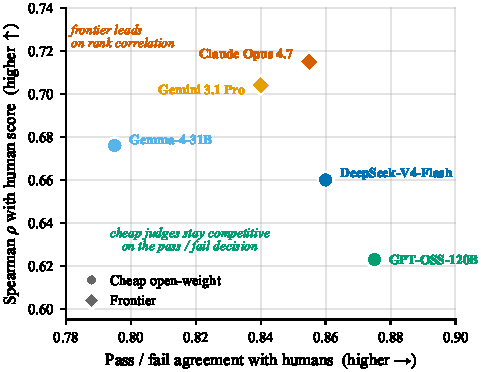
\includegraphics[width=0.86\columnwidth]{../../supplement/results/figures/figure5_passfail_vs_rank.pdf}
  \caption{Pass/fail agreement (x) versus Spearman rank correlation with the human
    score (y) on the validation sample ($n=200$). Cheap open-weight judges (circles)
    stay competitive on the pass/fail decision; the frontier baselines (diamonds) lead
    on rank correlation by a modest margin.}
  \label{fig:passrank}
\end{figure}

\end{document}
